Praca opiera się na~wykorzystaniu języka R \cite{strR} oraz Python \cite{strPython} do generowania zbiorów danych,
wszelkich manipulacji na~nich oraz ich klasyfikacji.

\section{Język R}

\begin{figure}[ht]
	\centering
	
\includegraphics[height=1.5cm]{resources/technologies/images/logo_r.png}
	\caption{Logo R \cite{strR}}
	\label{Fig:tech-r}
\end{figure}
\FloatBarrier

Język R~to szeroko stosowany w~statystyce, analizie danych oraz naukach przyrodniczych język interpretowalny.
Nie ma on skomplikowanej składni i~jest przystosowany do bycia jak najbardziej przyjaznym dla nowego użytkownika.
Oprócz dużych możliwości obliczeniowych, jest również świetnym narzędziem do wizualizacji danych,
co spowodowało, że został wybrany do stworzenia zbioru danych.
Grafy wygenerowane zostały przy pomocy biblioteki igraph \cite{strIgraph} w~wersji~2.0.3.
Jest to~pakiet do tworzenia i~analizy struktur sieci, a~co za tym idzie oferuje bogaty wybór funkcji do
generowania losowych i~regularnych grafów oraz ich wizualizacji.

\clearpage

\section{Język Python}

\begin{figure}[ht]
	\centering
	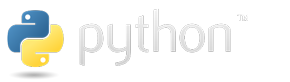
\includegraphics[height=1.5cm]{resources/technologies/images/logo_python.png}
	\caption{Logo Python \cite{strPython}}
	\label{Fig:tech-python}
\end{figure}
\FloatBarrier

Język Python jest jednym z~najpopularniejszych języków wysokopoziomowych ogólnego przeznaczenia.
Zawdzięcza to~swojej wszechstronności oraz prostocie składni.
Znaczna liczba bibliotek pozwala na~wykorzystywanie Pythona od
prostych skryptów, przez analizę danych, aż po rozbudowane aplikacje, takie jak całe
systemy największych gigantów technologicznych, np. Google. Język ten jest szeroko
wykorzystywany w~dziedzinie Data Science do wizualizacji, analizy~i przetwarzania danych oraz w~uczeniu maszynowym.
Ostatnie z~wymienionych zastosowań zadecydowało~o wyborze języka Python jako narzędzia do stworzenia modelu klasyfikacji grafów.
Wykorzystana została biblioteka Keras z~pakietu Tensorflow \cite{strTensorFlow}.
Do wizualizacji danych wykorzystana została biblioteka Matplotlib \cite{strMatplotlib}.

\section{Stanowisko pracy}
Całość pracy, tj. generacja danych, modele oraz testy, została przygotowana na~komputerze osobistym o~parametrach:

\begin{itemize}[label=-,labelsep=0.4cm,leftmargin=0.6cm]
\item CPU: i5-10400F 2.9 GHz
\item RAM: 32 GB 3200 MHz
\item GPU: ADM Radeon RX 5600 XT 6GB
\item Dysk: 2 x 1 TB HDD, 1 TB NVMe, 120 GB SSD
\item System operacyjny: Windows 10
\end{itemize}
System nie posiada karty graficznej zoptymalizowanej pod zastosowania uczenia maszynowego.
Biblioteki języka Python obsługują jednak karty graficzne AMD, co umożliwia pracę.